%%!TEX encoding = UTF-8 Unicode

% According to UA rules, font size should range from 10 to 12pt.
\documentclass[12pt,a4paper,openright,final,twoside,onecolumn]{memoir}

\listfiles
\fixpdflayout

\usepackage[utf8]{inputenc}

% Computer Modern Typewritter (For bold ttfamily in listings)
\usepackage{lmodern}
% OR... Bera Mono
%\usepackage[scaled]{beramono} % TTT Font
%\usepackage{anyfontsize} % As the name says...

\usepackage[T1]{fontenc}

% For Overleaf support
\usepackage{ifthen}
\def\useoverleaf{0}  % change to non-zero (for instance, 1) to enable it

\makeatletter
\newcommand{\makecoverfile}[0]{%
  \immediate\write18{latexmk -pdf cover.tex}%
}
\makeatother

%For PDF merging
\usepackage{pdfpages}

%SET DPI to 300
\pdfpxdimen=\dimexpr 1in/300\relax

\usepackage{morewrites} % Allow the use of a larger number of packages

%For English and Portuguese languages
%Portuguese will be the default.
%Use \setdefaultlanguage to change it
\usepackage{csquotes}
\usepackage[portuguese,english]{babel}


% For custom date format
\usepackage{datetime}
\newdateformat{thesisdate}{\monthname[\THEMONTH] \THEYEAR} % Month Year

\usepackage{microtype} % Make pdf look better


% Uncomment to enable floats on facing pages
%\usepackage{dpfloat}

%Side by side figures
% Eg. Fig 1a, Fig 1b
\usepackage[hang,small,bf]{caption}
%\let\tion\undefined
%\let\subfloat\undefined
\usepackage{subcaption}

%\RequirePackage{textcase}

% Dropped Caps
%\usepackage{lettrine}

% Configure Hyperlink color
%\usepackage[breaklinks=true,colorlinks=false,linkcolor=blue]{hyperref}
% Or use the default
\usepackage{hyperref}

%Optional: Redefine section names
%\def\sectionautorefname{Section}
%\def\chapterautorefname{Chapter}
%\def\figureautorefname{Figure}
%\def\listingautorefname{Listing}
%\def\tableautorefname{Table}

%For PDF Comments
\usepackage{comment}
\usepackage{pdfcomment}
\usepackage{bookmark} % New Bookmarks

%For Multiple columns in Glossary
\usepackage{multicol}

%Math symbols
\usepackage{mathtools}
\usepackage{amsmath}
\usepackage{amssymb}
\DeclareMathOperator*{\argmax}{arg\,max}
\DeclareMathOperator*{\argmin}{arg\,min}
\DeclareMathOperator*{\mode}{mode}

%Graphics
\usepackage{graphicx}

%Colors
\usepackage{xcolor}

%Euro symbol
\usepackage{eurosym}

% Code boxes
\ifthenelse{\equal{\useoverleaf}{0}}
{\usepackage[outputdir=build]{minted}}
{\usepackage{minted}}%

%\renewcommand\listingscaption{Código}
\fvset{fontsize=\footnotesize} % Make Code blocks smaller than text

%Biber using IEEE style for proper UTF-8 support
\usepackage[backend=biber,style=ieee, sorting=none]{biblatex}
\bibliography{bib/references.bib, bib/rfc.bib}

%Use acronyms
\usepackage[printonlyused]{acronym} % For acronyms

% Enable chart support through pgf and tikz
\usepackage[version=0.96]{pgf}
\usepackage{tikz}
\usepackage{pgf-umlsd}
\usetikzlibrary{arrows,shadows,trees,shapes,snakes,automata,backgrounds,petri,mindmap} % for pgf-umlsd

%For Electric Circuits
\usepackage[detect-weight=true, binary-units=true]{siunitx}
\sisetup{load-configurations = binary}

\usepackage[american,cuteinductors,smartlabels]{circuitikz}

\usetikzlibrary{calc}
\ctikzset{bipoles/thickness=1}
\ctikzset{bipoles/length=0.8cm}
\ctikzset{bipoles/diode/height=.375}
\ctikzset{bipoles/diode/width=.3}
\ctikzset{tripoles/thyristor/height=.8}
\ctikzset{tripoles/thyristor/width=1}
\ctikzset{bipoles/vsourceam/height/.initial=.7}
\ctikzset{bipoles/vsourceam/width/.initial=.7}
\tikzstyle{every node}=[font=\small]
\tikzstyle{every path}=[line width=0.8pt,line cap=round,line join=round]

% For inline TT text (e.g. code snippets)
\usepackage{verbatim}

 %Frames around figures and allow force placement
\usepackage{float}

%Configure Float style
%\floatstyle{boxed}
%\restylefloat{table}
%\restylefloat{figure}
%\restylefloat{lstlisting}

%For test purposes
\usepackage{lipsum}

%Keep floats inside section!
\usepackage[section]{placeins}
\let \oldsubsubsection \subsubsection
\renewcommand{\subsubsection}[2][]{
  \FloatBarrier
  \oldsubsubsection#1{#2}
}
\let \oldsubsection \subsection
\renewcommand{\subsection}[2][]{
  \FloatBarrier
  \oldsubsection#1{#2}
}
\let \oldsection \section
\renewcommand{\section}[2][]{
  \FloatBarrier
  \oldsection#1{#2}
}
\let \oldchapter \chapter
\renewcommand{\chapter}[2][]{
  \FloatBarrier
  \oldchapter#1{#2}
}


%%%% Use the built-in division styling
\headstyles{memman}

%%% ToC down to subsections
\settocdepth{subsection}

%%% Numbering down to subsections as well
\setsecnumdepth{subsection}

%%%% extra index for first lines
\makeindex[lines]

%Margins for University of Aveiro Thesis
\setlrmarginsandblock{3cm}{2.5cm}{*}
\setulmarginsandblock{3cm}{3cm}{*}
\checkandfixthelayout

%Or custom spacing
%\addtolength{\parskip}{0.5\baselineskip}
\linespread{1.5}

\begin{document}
\ifthenelse{\equal{\useoverleaf}{0}}{}{\makecoverfile{}}%
\includepdf[pages=-]{cover.pdf}

%
%Front matter

%Custom Chapter style named thesis
\makechapterstyle{thesis}{% Based on ell
  \chapterstyle{default}
  \renewcommand*{\chapnumfont}{\normalfont\sffamily}
  \renewcommand*{\chaptitlefont}{\normalfont\Huge\sffamily}
  \settowidth{\chapindent}{\chapnumfont 111}
  \renewcommand*{\chapterheadstart}{\begingroup
    \vspace*{\beforechapskip}%
    \begin{adjustwidth}{}{-\chapindent}%
    \hrulefill
    \smash{\rule{0.4pt}{15mm}}
    \end{adjustwidth}\endgroup}
  \renewcommand*{\printchaptername}{}
  \renewcommand*{\chapternamenum}{}
  \renewcommand*{\printchapternum}{%
    \begin{adjustwidth}{}{-\chapindent}
    \hfill
    \raisebox{10mm}[0pt][0pt]{\fontsize{30}{25}\selectfont\chapnumfont \thechapter}%
                              \hspace*{1em}
    \end{adjustwidth}\vspace*{-3.0\onelineskip}}
  \renewcommand*{\printchaptertitle}[1]{%
    \vskip\onelineskip
    \raggedleft {\chaptitlefont ##1}\par\nobreak\vskip 4\onelineskip}}


%Select chapter style from existing or select custom
%\chapterstyle{thesis} % Others: dowding, demo2, dash, chappell, brotherton, bianchi, ger, madsen, tatcher, veelo,indexes)
% thesis can also be used as defined previously
%

%If you feel adventurous you can also define all aspects of your theme
%Use either this input or the chapterstyle before
%% Rules
\newcommand{\thinRule}{\rule{\textwidth}{0.25pt}}

% Customize heading appearances
% Define styles
\newcommand{\partSize}{\Huge}
\newcommand{\partStyle}{\lsstyle\scshape}
\newcommand{\chapterSize}{\Huge}
\newcommand{\chapterStyle}{\lsstyle\scshape}
\newcommand{\chapterAfter}{}
\newcommand{\sectionSize}{\Large}
\newcommand{\sectionStyle}{\scshape\MakeTextLowercase}
\newcommand{\subsectionSize}{\large}
\newcommand{\subsectionStyle}{\scshape\MakeTextLowercase}
\newcommand{\subsubsectionSize}{\large}
\newcommand{\subsubsectionStyle}{\scshape\MakeTextLowercase}
\newlength{\partNumSizePt}
\setlength{\partNumSizePt}{60pt}
\newlength{\chapterNumSizePt}
\setlength{\chapterNumSizePt}{60pt}
\newcommand{\partNumSize}{%
  \fontsize{\partNumSizePt}{1.2\partNumSizePt}\selectfont%
}
\newcommand{\partNumStyle}{\partChapterNumColor}
\newcommand{\chapterNumSize}{%
  \fontsize{\chapterNumSizePt}{1.2\chapterNumSizePt}\selectfont%
}
\newcommand{\chapterNumStyle}{\partChapterNumColor}

% Customize parts
\renewcommand{\partnamefont}{\partSize\partStyle}
\renewcommand{\partnumfont}{\partNumSize\partNumStyle}
\renewcommand{\printpartname}{}
\renewcommand{\printparttitle}[1]{%
  \normalfont\normalcolor\partnamefont #1
}

% Customize chapters
\makeatletter
\setlength{\beforechapskip}{30pt}
\renewcommand*{\chapterheadstart}{\vspace*{\beforechapskip}}
\setlength{\afterchapskip}{3ex}
\setlength{\midchapskip}{3ex}
\renewcommand*{\chapnamefont}{%
  \Large\flushright\chapterStyle\partChapterNumColor%
}
\renewcommand*{\chapnumfont}{\chapterNumSize\chapterNumStyle}
\renewcommand*{\chaptitlefont}{%
  \normalfont\flushleft\normalcolor\chapterSize\chapterStyle%
}
\renewcommand*{\printchaptername}{%
  \chapnamefont\MakeTextLowercase{\@chapapp}%
}
\renewcommand*{\chapternamenum}{\quad}
\renewcommand*{\printchapternum}{%
%  \chapnumfont\textls[-75]{\classicstylenums{\thechapter}}%
 \chapnumfont\textls[-75]{\thechapter}%

}
\renewcommand*{\printchaptertitle}[1]{%
  \chaptitlefont #1
  \chapterAfter
}
\makeatother
% Customize sections and subsections
\setsecnumformat{\csname my#1\endcsname\quad}
\setsecheadstyle{\sectionSize\sectionStyle}
\newcommand{\mysection}{{\thesection}}
\setlength{\beforesecskip}{3em}


\setsubsecheadstyle{\subsectionSize\subsectionStyle}
\newcommand{\mysubsection}{{\normalfont\subsectionSize\thesubsection}}
\setlength{\beforesubsecskip}{3em}

\setsubsubsecheadstyle{\subsubsectionSize\subsubsectionStyle}
\newcommand{\mysubsubsection}{{\normalfont\subsubsectionSize\thesubsubsection}}
\setlength{\beforesubsubsecskip}{2em}

% Customize "Table of ..." appearance
% Customize headings
\newcommand{\renewPrintXTitle}[1]{%
  \renewcommand{#1}[1]{%
    \printchaptertitle{##1}%
  }%
}
\renewPrintXTitle{\printtoctitle}
\renewPrintXTitle{\printlottitle}
\renewPrintXTitle{\printloftitle}

% Customize ToC headings
\renewcommand{\cftpartfont}{\partChapterNumColor\partStyle}
\renewcommand{\cftchapterfont}{\chapterStyle}
\renewcommand{\cftsectionfont}{}
\renewcommand{\cftsubsectionfont}{}
\renewcommand{\cftfigurefont}{}
\renewcommand{\cfttablefont}{}
\newcommand{\cftlstlistingfont}{}

% Increase number width
\newlength{\cftNumWidthIncrease}
\setlength{\cftNumWidthIncrease}{0.25em}
\addtolength{\cftpartnumwidth}{\cftNumWidthIncrease}
\addtolength{\cftchapternumwidth}{\cftNumWidthIncrease}
\addtolength{\cftsectionindent}{\cftNumWidthIncrease}
\addtolength{\cftsubsectionindent}{\cftNumWidthIncrease}
% No leader dots
%\renewcommand*{\cftpartdotsep}{\cftnodots}
%\renewcommand*{\cftchapterdotsep}{\cftnodots}
%\renewcommand*{\cftsectiondotsep}{\cftnodots}
%\renewcommand*{\cftsubsectiondotsep}{\cftnodots}
%\renewcommand*{\cftfiguredotsep}{\cftnodots}
%\renewcommand*{\cfttabledotsep}{\cftnodots}
%\newcommand*{\cftlstlistingdotsep}{\cftnodots}
% Set page numbers immediately after entry text
\newcommand{\tocEntryPageSep}{\hspace{1em}}
\renewcommand{\cftpartleader}{\cftdotfill{\cftdotsep}}
%\renewcommand{\cftpartafterpnum}{\cftparfillskip}
%\renewcommand{\cftchapterleader}{\tocEntryPageSep}
\renewcommand{\cftchapterleader}{\cftdotfill{\cftdotsep}}
%\renewcommand{\cftchapterafterpnum}{\cftparfillskip}
\renewcommand{\cftsectionleader}{\cftdotfill{\cftdotsep}}
%\renewcommand{\cftsectionafterpnum}{\cftparfillskip}
\renewcommand{\cftsubsectionleader}{\cftdotfill{\cftdotsep}}
%\renewcommand{\cftsubsectionafterpnum}{\cftparfillskip}
\renewcommand{\cftfigureleader}{\cftdotfill{\cftdotsep}}
%\renewcommand{\cftfigureafterpnum}{\cftparfillskip}
\renewcommand{\cfttableleader}{\cftdotfill{\cftdotsep}}
%\renewcommand{\cfttableafterpnum}{\cftparfillskip}
\newcommand{\cftlstlistingleader}{\cftdotfill{\cftdotsep}}
%\newcommand{\cftlstlistingafterpnum}{\cftparfillskip}
% Customize page numbers
\newcommand{\tocPageStyle}{\tocPageColor}
\renewcommand{\cftpartpagefont}{\tocPageStyle}
\renewcommand{\cftchapterpagefont}{\tocPageStyle}
\renewcommand{\cftsectionpagefont}{\tocPageStyle}
\renewcommand{\cftsubsectionpagefont}{\tocPageStyle}
\renewcommand{\cftfigurepagefont}{\tocPageStyle}
\renewcommand{\cfttablepagefont}{\tocPageStyle}
\newcommand{\cftlstlistingpagefont}{\tocPageStyle}

% Abstract
% Remove indents around abstract text
\setlength{\absleftindent}{0pt}
\setlength{\absrightindent}{0pt}
% Change font size to conform with the rest of the document text
\renewcommand{\abstracttextfont}{\normalsize}

% Customize headers and footers including page numbers
\newcommand{\hfTextSize}{\footnotesize}
\newcommand{\headTextStyle}{\lsstyle\scshape\MakeTextLowercase}
\nouppercaseheads
\makeevenhead{headings}%
             {\hfTextSize\thepage}%
             {}%
             {\hfTextSize\headTextStyle\leftmark}
\makeevenhead{plain}%
             {\hfTextSize\thepage}%
             {}%
             {\hfTextSize\headTextStyle\leftmark}
\makeoddhead{headings}%
            {\hfTextSize\headTextStyle\rightmark}%
            {}%
            {\hfTextSize\thepage}
\makeoddhead{plain}%
            {\hfTextSize\headTextStyle\rightmark}%
            {}%
            {\hfTextSize\thepage}


% Customize captions
\newcommand{\captionSize}{\small}
\newcommand{\captionStyle}{\scshape}
\newcommand{\captionWidthRatio}{0.9}

\captionnamefont{\captionSize\captionStyle}
\captiontitlefont{\captionSize}
\captiondelim{ -- }
\captiontitlefinal{}
\changecaptionwidth
%\captionwidth{\captionWidthRatio\textwidth}

% Define colors
%\newcommand{\titleColor}{\color[rgb]{0.616, 0.0627, 0.176}}
\newcommand{\titleColor}{\color[rgb]{0,0,0}}

\newcommand{\partChapterNumColor}{\titleColor}
\newcommand{\dropCapColor}{\titleColor}
%\newcommand{\tocPageColor}{\color[rgb]{0.0980, 0.329, 0.651}}

\newcommand{\tocPageColor}{\color[rgb]{0, 0,0}}
\definecolor{shade0}{rgb}{1.0 , 1.0 , 1.0 }
\definecolor{shade1}{rgb}{0.9 , 0.9 , 0.9 }
\definecolor{shade2}{rgb}{0.8 , 0.8 , 0.8 }
\definecolor{shade3}{rgb}{0.65, 0.65, 0.65}
\definecolor{shade4}{rgb}{0.45, 0.45, 0.45}
\definecolor{shade5}{rgb}{0.0 , 0.0 , 0.0 }



\chapterstyle{veelo}
%Exclude sub figures from List of Figures
%\captionsetup[subfloat]{list=no}


% Texts
\newenvironment{introduction}
{%
  \begin{minipage}{\textwidth}%
   \itshape%
}
{%
  \end{minipage}%
  \par\addvspace{2\baselineskip plus 0.2\baselineskip minus 0.2\baselineskip}%
}


%Select Page style
\pagestyle{plain}

\frontmatter

\tightlists
\midsloppy
\raggedbottom

\setcounter{tocdepth}{2} %subsections are added to the TOC
\setcounter{secnumdepth}{4} %subsubsections are numbered


\cleardoublepage

%Table of contents
{\small\tableofcontents}
\cleardoublepage

%List of figures
{\small\listoffigures}


%List of tables
\cleardoublepage
{\small\listoftables}

%Print Glossary
{\small\chapter{Glossary}

\footnotesize
\SingleSpacing

\begin{multicols}{2}
\begin{acronym}[AAAAAA]

	\acro{DL}[DL]{Deep Learning}
	\acro{ANN}[ANN]{Artificial Neural Network}
	\acro{CNN}[CNN]{Convolutional Neural Network}
	\acro{GPU}[GPU]{Graphics Processing Unit}
	\acro{CPU}[CPU]{Central Processing Unit}
	\acro{SGD}[SGD]{Stochastic Gradient Descent}
	\acro{PRNG}[PRNG]{Pseudo Random Number Generator}

\end{acronym}
\end{multicols}
}

%
%Main document starts here
%
\mainmatter



% Start of Thesis text ----------------------------------------------------------
%Line spacing: 1.5 pt
\OnehalfSpacing

\chapter{Introduction}
\label{chapter:introduction}

This introductory chapter introduces this dissertation's motivation, objectives, and high-level outline.

\section{Motivation}

Melanoma is a cancer that is developed from melanocytes, i.e. cells that produce the melanin skin pigment. This abnormal growth of tissue generally occurs in skin, but can also manifest itself in the mouth, intestines or eyes. The most common cause of melanoma is the exposure to ultraviolet light (e.g. sunlight, tanning devices), thus it can be prevented by frequent use of sunscreen and avoiding long exposure to the sun. The clinical diagnosis is confirmed with a skin biopsy and, if it hasn't spread, treatment is usually surgical excision.

Melanoma is a dangerous type of skin cancer which, in 2012, occurred in 232000 people, and in 2015 there were 3.1 million people with the disease that resulted in over 59000 deaths worldwide. According to the \ac{CDC} , the rates of new melanomas have doubled over the last three decades and will continue to double.

Since the skin lesions occur on the surface of the skin, melanoma can easily be detected early through visual inspection by a physician with the use of dermoscopy techniques that allow a better look at the pigmented lesions. Dermoscopy is an imaging technique that works by removing the surface reflection of the skin which enables the visualization of enhanced levels of skin. More recently, computerized digital dermoscopy has made it relatively trivial to get high resolution imaging that can be used to get second opinions remotely or even a computer-assisted diagnosis\cite{dermoscopy}. More specifically, advances in deep learning algorithms and computer hardware has made classification by a machine learning algorithm a viable and reliable technique for a diagnosis.

Deep learning architectures are an improvement of \ac{ANN} characterized by the large number of hidden processing layers capable of learning hierarchical feature representations. One major advantage of deep learning is that it reduces the need of feature engineering, which is one of the most complicated and time consuming parts in machine learning practice. The successes of deep learning architectures are now well reported in computer vision. The latest developments have been boosted by the use of \ac{GPU} to speedup computations and the development of high-level modules to build neural networks such as Theano, Caffe and TensorFlow.

The surveys by Greenspan, Ginneken and Summers \cite{intro1}, Hu et al. \cite{intro2} and Litjens et al. \cite{intro3} contribute to a clear understanding of the principles and methods of neural networks and deep learning applied to medical image analysis. They provide insight into how the algorithms based on deep models, namely \ac{CNN}, are being applied in different contexts, such as organ segmentation, lesion detection or tumor classification. A particular area where deep learning is rapidly improving the state-of-the art is in dermatology care \cite{nature2017}\cite{intro5}\cite{intro6}. The results achieved are impressive despite the many challenges for training deep models with many layers composed by adaptive parameters encompass.

The first challenge is that deep learning models often require a large amount of training data to achieve superior performance than other methods (shallow competitors). Second, the objective function is often a highly non-convex function of the parameters with the potential for local minima. Third, we still lack the right methodology to fully comprehend the deep structure of a trained model that works, to a large extent, like a black box. Consequently, training deep models from scratch requires large amounts of annotated data and massive computational resources. Transfer learning has emerged as a promising solution to the data challenge by using, as baseline, the knowledge from a deep model previously trained on a large labelled dataset \cite{intro7}\cite{howtransferable}\cite{intro9}.

\section{Objectives}

The objective is to assess and compare the effectiveness of transfer learning in the specific domain of skin lesion classification by running experiments that will train and evaluate models using various different techniques.

The first set of experiments focuses on transfer learning. In general, we start from models previously trained on ImageNet (of a variety of architectures) and repurpose them for the task of skin lesion classification by extracting weights from arbitrary layers and continuing training on our dataset. Namely in our study we consider as a variable the layer where this extraction of weights occurs and study its effect.

The second set of experiments focuses on a simpler custom \ac{CNN} architecture designed around first-principle heuristics and trained end-to-end, rather than the transfer learning approach of initializing the weights to those of the pre-trained model, thus presenting a model obtained by following more traditional techniques for comparison.

\section{Outline}

At a high level, this dissertation is organized into 5 other chapters:

\begin{itemize}
    \item Chapter \ref{chapter:background} introduces the reader to deep learning concepts and state-of-the-art techniques relevant to this dissertation;
    \item Chapter \ref{chapter:sota} reviews the state-of-the-art results of deep learning applied to dermoscopy;
    \item Chapter \ref{chapter:environment} introduces the hardware and software used for this work;
    \item Chapter \ref{chapter:experiments} goes over this work's methodology and presents and discusses the experimental results;
    \item Chapter \ref{chapter:conclusion} offers final remarks, key takeaways, and points in the direction of future work.
\end{itemize}

\chapter{Background}
\label{chapter:background}

This chapter provides the necessary background of machine learning and deep learning to better familiarize the reader with the techniques as well as contextualize the state-of-the-art work that will be reviewed later in chapter \ref{chapter:sota}.

\section{Supervised Learning}

A supervised learning problem is a machine learning problem in which the data has the correct expected output for every input.

More formally, it is a problem in which there are $m$ labeled pairs $(x^{(i)}, y^{(i)})$, also denoted as samples, where $x^{(i)} \in \mathbb{R}^n$ (i.e. the input vectors, commonly referred to as features) and $y^{(i)} \in \mathbb{R}^n$ (i.e. the corresponding output vector, usually called the target or label) which have some relationship expressed by some function.

The goal of supervised learning is to find a function $h_{\theta}(x)$ (sometimes called the hypothesis) that usefully approximates the true function in the underlying relationship between the input $x$ and associated output $y$, parameterized by $\theta$.

In supervised learning, the data samples are commonly split into three separate sets with different intents and used exclusively for that purpose:

\begin{itemize}
    \item Training Set: samples used for actually fitting the model's parameters (e.g. weights and biases of a neural network);
    \item Validation Set: samples used to select the best model by testing different sets of hyperparameters or architectures;
    \item Test Set: samples used to assess the final performance of the final model.
\end{itemize}

It is important to follow this taxonomy carefully and not use the different sets for the different tasks interchangeably. As \citeauthor{crossvalidationbias} point out in their \citeyear{crossvalidationbias} paper, if, for example, we use the test set to simultaneously tune hyperparameters and assess its generalization performance we risk optimistically biasing the model. As such, if we use any one set to tune hyperparameters, we must use a different set for evaluation to get an unbiased assessment of the model's generalization performance.

However, this technique (typically referred to as the holdout method) has its downsides:

\begin{itemize}
    \item using an arbitrary fixed split of the dataset means that we are completely setting aside data for validation and testing which will not be used for fitting the model and vice versa, thus wasting data in some sense
    \item without averaging over multiple runs (i.e. different splits) with different initial conditions, results may be biased and misleading
\end{itemize}

$K$-fold cross-validation is a common cross-validation technique that randomly partitions the data into $K$ equally sized subsamples, of which a single subsample is used for testing and the remaining $K-1$ subsamples for fitting the model, a process which is repeated $K$ times to yield $K$ performance estimations that can be averaged over to produce one estimation that can be referred to. In this way all samples are used for training and testing, which is an advantage over repeated random sub-sampling which does not systematically use all samples for training and testing.

Nested cross-validation techniques are required when, in addition to estimating a model's generalization performance (i.e. performance on the test set), it is also necessary to select the best model among many (e.g. with different hyperparameters) \cite{crossvalidationbias}. A truly nested variant will use an inner loop of $L$ folds to tune the hyperparameters and select the best model, and an outer loop of $K$ folds to evaluate the models selected by the inner loop. A simpler (albeit not really nested) scheme is one that is similar to the $K$-fold cross-validation we described above, except that, of the $K$ equally sized subsamples, we take 1 subsample for validation, another 1 subsample for testing, and the remaining $K-2$ subsamples are used for training. However, in practice, nested cross-validation when selecting classifiers is overzealous and too expensive for most applications \cite{nestedcvoverzealous}.

\section{Binary Classification}

In general, let

\begin{itemize}
    \item $L \colon \mathbb{R}^n \to \mathbb{R}$ be a function, called the loss function, which quantifies the quality of a particular set of parameters $\theta$ relative to a single data sample $(x^{(i)}, y^{(i)})$;
    \item $J \colon \mathbb{R}^n \to \mathbb{R}$ be a function, called the cost function, which quantifies the quality of a particular set of parameters $\theta$ relative to all the $m$ samples in the training set. $$J(\theta) = \frac{1}{m} \sum_{i=1}^{m} L(h_{\theta}(x^{(i)}), y^{(i)})$$
\end{itemize}

In particular, the linear regression cost function can be easily understood as the summation of the differences between the predictions and the ground truth labels:

$$
J(\theta) = \frac{1}{2m} \sum_{i=1}^{m} (h_{\theta}(x^{(i)}) - y^{(i)})^2
$$

In a binary classification problem specifically we have that $y^{(i)} \in \{0, 1\}$. Unfortunately, as it turns out, the linear regression cost function is unsuitable for binary classification because it would be a non-convex function with many local minima, which in turn would make optimization very difficult.

Essentially, binary classification requires a cost function that penalizes very confident wrong predictions while also rewarding confident right predictions, i.e.,

\begin{itemize}
    \item if the prediction is $h_{\theta}(x) = 0$ and the ground-truth label is $y = 0$, $J(\theta)$ is low;
    \item if the prediction is $h_{\theta}(x) = 0$ and the ground-truth label is $y = 1$, $J(\theta)$ is high;
    \item if the prediction is $h_{\theta}(x) = 1$ and the ground-truth label is $y = 0$, $J(\theta)$ is high;
    \item if the prediction is $h_{\theta}(x) = 1$ and the ground-truth label is $y = 1$, $J(\theta)$ is low.
\end{itemize}

Whereas in linear regression the hypothesis is of the form $h_{\theta}(x) = \theta^Tx$, in binary classification (or logistic regression) the hypothesis is of the form $h_{\theta}(x) = \sigma(\theta^Tx)$ to squash predictions to the interval $[0, 1]$, hence the name logistic regression, because it uses the sigmoid-shaped logistic function $\sigma(z) = \frac{1}{1 + e^{-z}}$.

A useful loss function (sometimes called binary cross-entropy in some literature) for logistic regression that takes these requirements into consideration is

$$
L(h_{\theta}(x^{(i)}), y^{(i)}) =
\begin{dcases}
    -\log(h_{\theta}(x^{(i)})),& \text{if } y^{(i)} = 1\\
    -\log(1 - h_{\theta}(x^{(i)})),& \text{if } y^{(i)} = 0
\end{dcases}
$$

or, cleverly arranging things algebraically,

$$
J(\theta) = -\frac{1}{m} \sum_{i=0}^{m} ( y^{(i)}\log(h_{\theta}(x^{(i)})) + (1 - y^{(i)})\log(1 - h_{\theta}(x^{(i)})) )
$$

\subsection{Evaluation}

To evaluate a binary classifier means to compare the model's predicted conditions against the true conditions, where one must consider:

\begin{itemize}
    \item \ac{TP}, cases correctly classified as positive, i.e. $h(x^{(i)}) = 1$ matches $y^{(i)} = 1$;
    \item \ac{TN}, cases correctly classified as negative, i.e. $h(x^{(i)}) = 0$ matches $y^{(i)} = 0$;
    \item \ac{FP}, cases incorrectly classified as positive, i.e. $h(x^{(i)}) = 1$ but $y^{(i)} = 0$;
    \item \ac{FN}, cases incorrectly classified as negative, i.e. $h(x^{(i)}) = 0$ but $y^{(i)} = 1$.
\end{itemize}

From these basic measurements one can derive useful metrics:

\begin{itemize}
    \item \ac{TPR}, also known as sensitivity or recall, is basically the percentage of actual positives that are correctly identified as positive;
        $$TPR = \frac{TP}{TP + FN}$$
    \item \ac{TNR}, also known as specificity, is the percentage of actual negatives that are correctly identified as negative;
        $$TNR = \frac{TN}{FP + TN}$$
    \item \ac{PPV}, also known as precision,
        $$PPV = \frac{TP}{TP + FP}$$
    \item \ac{NPV}
        $$NPV = \frac{TN}{TN + FN}$$
    \item \ac{FPR} is the percentage of actual positives that are incorrectly identified as negative;
        $$FPR = 1 - TNR$$
\end{itemize}

As a summary statistic one can derive the accuracy $A$ as the percentage of total items classified correctly

$$
A = \frac{TP + TN}{TP + FP + TN + FN}
$$

However accuracy is misleading in cases where there is a class imbalance because a model can always predict the value of the majority class and still report a high accuracy value despite missing all predictions in the minority class. Instead F1 score should be preferred. F1 score is the harmonic mean of precision and recall given by

$$
F_1 = 2 \times \frac{PPV \times TPR}{PPV + TPR}
$$

Lastly, \ac{AUC} is known as the area under the \ac{ROC} curve, i.e. the area under the plot of \ac{FPR} versus \ac{TPR} at different points in the interval $[0, 1]$.

\subsection{Class Imbalance}

In binary classification problems, it is said that a dataset of $m$ samples has class imbalance when there is a majority class with $|S_{maj}|$ samples and a minority class with $|S_{min}|$ samples where $|S_{maj}| > |S_{min}|$, in other words when there is a significant difference between the number of samples of one class compared to the other. It is very common to see datasets in which classes are highly imbalanced, simply because it reflects the real world distribution (e.g. there are more benign moles than actual melanoma cases). A lot of machine learning algorithms do not perform well under this imbalance. When a dataset is imbalanced, machine learning algorithms will typically over-classify the majority group due to its increased prior probability. Thus, the samples in the minority group are misclassified more often than the majority group \cite{Johnson2019}.

\citeauthor{haibo2009} provide a comprehensive survey of class balancing algorithms \cite{haibo2009}, of which oversampling of the minority class is the simplest and most natural. In practice the minority class must be oversampled by a factor (i.e. number of transformations applied to each original sample) of $\frac{|S_{maj}|}{|S_{min}|}$. Sometimes, perhaps because of an overfitting problem, it is also necessary to augment the total number of samples $m$ to a new total number of samples $m'$, in which case

\begin{itemize}
    \item the minority class must be oversampled by augmenting its samples  by a factor of $\frac{\frac{m'}{2}}{|S_{min}|}$
    \item and the majority class must also be augmented by a factor of $\frac{\frac{m'}{2}}{|S_{maj}|}$
\end{itemize}

\section{Optimization}

Given a cost function $J$ and initial parameters $\theta$, the goal is to find the optimal $\theta^*$ that minimizes the cost function, i.e. the optimization objective is

$$
\theta^{*} = \argmin_{\theta} J(\theta)
$$

In the deep learning high-dimensional optimization landscape, the objective function is highly non-convex w.r.t. the parameters, so one can't use any of the tools from the convex optimization literature. Using calculus to find the minimum analytically is only feasible for trivial, low-dimensional, convex functions.

\subsection{Brute-force Search}

A naive first approach is to systematically and exhaustively enumerate and evaluate many candidate solutions while keeping track of the best one. This simple solution, arguably the simplest metaheuristic, is infeasible in the context of deep neural networks due to the curse of dimensionality.

\subsection{Random Optimization}

Rather than try all solutions exhaustively, another approach is to try random values of $\theta$ in a loop and record the running best until some stopping criteria.

\subsection{Random Local Search}

A slightly better strategy is to start with random $\theta$ and iteratively refine the best-found solution (hence the local in local search) until some stopping criteria.

\subsection{Gradient Descent}

Random local search forms a good basis for optimization, but there is no need to move randomly in search-space. The negative of the gradient of the cost function w.r.t. the parameters $\theta$ over all $m$ training samples gives the direction of steepest descent (i.e. the direction in which the cost function decreases):

$$
\nabla_{\theta} J(\theta) = \frac{1}{m} \sum_{i=1}^{m} \nabla_{\theta} L(h_{\theta}(x^{(i)}), y^{(i)})
$$

A parameter $\eta \in \mathbb{{R}^{+}}$, called the learning rate, controls the size of the step to take in the direction of the gradient. The learning rate $\eta$ must be set carefully to ensure that the cost function converges. A small enough value will ensure convergence, but requires a larger number of updates to get there, whereas bigger values will likely result in divergence. The learning rate can also be set dynamically to change during training. One such heuristic is to reduce it by a factor $f$ (e.g. $f=0.1$) when the loss has not changed significantly within some threshold $\epsilon$ (e.g. $\epsilon=0.0001$) in $p$ epochs (e.g. $p=30$) during which it will be patient \cite{learningrateschedules}.

Thus emerges a very simple and natural update rule (called batch gradient descent) for our parameters:

$$
\theta^{t+1} = \theta^t - \eta \nabla_{\theta} J(\theta)
$$

Computing the gradient $\nabla J$ with respect to the original $m$ training samples is computationally and memory intensive for very big $m$. But, as it turns out, through an idea interchangeably referred to as mini-batch gradient descent or \ac{SGD}, we can get a good estimate of the true gradient $\nabla J$, by averaging over a smaller random number of samples $m'$, i.e.,

$$
\nabla J \approx \frac{\sum_{i=1}^{m'} \nabla J_i}{m'} \approx \frac{\sum_{i=1}^m \nabla J_{i}}{m}
$$

A variation of \ac{SGD} called \ac{SGD} with momentum \cite{ruder2016} keeps track of the past parameter updates in a vector $v$ (with $\dim v = \dim \theta$) which initially, at iteration $t = 0$, is the zero matrix

$$
v^0 = 0
$$

and $v^{t+1}$ holds a fraction $\gamma \in [0,1]$ (usually $\gamma = 0.9$) of the updates up until iteration $t$, i.e.,

$$
v^{t+1} = -\eta \nabla_{\theta} J(\theta) + \gamma v^{t}
$$

and determines that the parameter update at (the next) iteration $t+1$ is a linear combination of the gradient and the previous parameter updates $v^{t}$:

\begin{align*}
    \theta^{t+1} &= \theta^{t} + v^{t+1} \\
                 &= \theta^{t} - \eta \nabla_{\theta} J(\theta) + \gamma v^{t}
\end{align*}

\ac{SGD} with momentum effectively helps accelerate \ac{SGD} in the relevant direction and dampen oscillations in the parameter values \cite{ruder2016}.

More recently, adaptive gradient descent methods have been further developed to find individual learning rates per parameter and use ideas similar to momentum, which \citeauthor{ruder2016} \cite{ruder2016} presents an extensive review of. Despite the popularity of these adaptive methods (e.g. Adam), sometimes they offer marginal value versus the classic \ac{SGD}. Wilson et al. \cite{wilson2017} show that the solutions found by adaptive methods usually generalize worse when compared to \ac{SGD}, which suggests that adaptive methods like Adam should not be used like a magical black box but cross-validated among other optimizers.

% TODO: https://www.i2tutorials.com/technology/back-propagation-and-computational-graphs-in-neural-networks/
% TODO: http://outlace.com/on-chain-rule-computational-graphs-and-backpropagation.html
\section{Computational Graphs}

In some sense, a neural network is just an arbitrarily composite function.

$$
f(x) = g(h( ... j(x) ... ))
$$

Such a function can be represented in a directed acyclic graph (which the machine learning literature calls a computational graph) where each node in the graph is a variable (which can be a scalar blabla) and an edge is an operation, e.g. $f(x) = x+2$ would draw two nodes ($x$ and $2$) connected by an edge (the addition operator).

On a computational graph we can have essentially two types of computation:

\begin{itemize}
    \item Forward propagation (i.e. inference) runs an input $x$ through this arbitrarily composed function.
    \item Backward propagation is all about understanding how changing one variable affects another, which computational graphs make quite easy.
\end{itemize}

Computational graphs expose a programming model where the big idea is to express a numeric computation as a graph and

\begin{itemize}
    \item graph nodes are operations which have any number of inputs and outputs;
    \item graph edges are tensors that flow between nodes.
\end{itemize}

Computational graphs also make it easy to move computation to GPU or TPU [citation needed].

\section{Initialization}

An optimization algorithm like gradient descent is inherently iterative in its update rule (for iterations $t > 0$)

$$
\theta^{t+1} = \theta^t - \eta \nabla_{\theta} J(\theta)
$$

for which we need to initialize the matrix $\theta^0$ such that the first update works. This initialization determines how quickly optimization converges or whether it converges at all, which is why it is so important.

A reasonable first approach would be to initialize all values of the matrix $\theta$ to zero. However, e.g. in a neural network this does not have any symmetry breaking properties because if every weight is initialized to zero then every neuron will compute the same activation (assuming all neurons use the same activation function), thus the gradients computed by backpropagation will also be the same and result in the exact same updates during gradient descent. Therefore parameters must be chosen in such a way that they break this symmetry, which is what motivates the use of random initialization. However simply drawing random parameters (e.g. from a Gaussian distribution with mean 0 and standard deviation 1) might result in too small or too big parameter values and very wide in range which originate a vanishing or exploding gradient problem where different layers effectively learn at different speeds.

Modern initialization techniques are heuristic based and designed around the activation functions themselves to counter these problems by, essentially, guaranteeing the activations' mean to be $0$ and the variance to be the same across different layers. Under these conditions the backpropagated gradient will not be multiplied by very small or very big values (which would lead to vanishing or exploding gradient problems, respectively). Specifically,

\begin{itemize}
    \item for tanh activation functions, Xavier et al. \cite{xavierinit} recommend drawing parameters from either $\mathcal{N}(0, \frac{1}{n_{in}})$ or $\mathcal{N}(0, \frac{2}{n_{in}+n_{out}})$ where $n_{in}$ is the number of input neurons and $n_{out}$ the number of output neurons in that layer;
    \item for ReLU activation functions, He et al. \cite{heinit} suggest drawing from $\mathcal{N}(0, \frac{2}{n_{in}})$.
\end{itemize}

More recently, initializing a network with parameters transferred from other networks (typically trained on natural image datasets whose lower-layers' features generalise well to other tasks) has emerged as a very useful and pragmatic initialization strategy which in practice works very well for most tasks \cite{howtransferable}, giving birth to what is now known as transfer learning.

\section{Feature Normalization}

Some machine learning algorithms rely on the distance between the features in a feature vector $x$ and assume the values are on the same scale. Min-max normalization rescales $x$ to $x'$ to be on the interval $[0, 1]$, i.e.

$$
x' = \frac{x - \min{(x)}}{\max{(x)} - \min{(x)}}
$$

Other machine learning algorithms assume that the feature vector $x$ follows a Gaussian distribution (i.e. zero mean and unit-variance). Gaussian normalization is the process of rescaling $x$ (where $\mu_x$ is the mean of each feature vector $x$ and $\sigma_x$ its standard deviation) to $x'$ to follow a Gaussian distribution, i.e.

$$
x' = \frac{x - \mu_x}{\sigma_x}
$$

In practice, gradient descent converges much faster with features that follow a normal distribution as was seen by the work of \citeauthor{batchnormalization} on batch normalization \cite{batchnormalization}.

Performing feature normalization on the entire dataset and only afterwards split it (into train, validation, and test sets) will leak information (i.e. the mean and variance) about the validation and test sets into the train set itself which will bias performance metrics on the validation and test sets. Therefore, it is crucial to

\begin{enumerate}
    \item Split the dataset;
    \item Perform feature normalization on the train set and save the mean $\mu_{train}$ and variance $\sigma_{train}$;
    \item Perform feature normalization on the validation set using the mean $\mu_{train}$ and variance $\sigma_{train}$;
    \item Perform feature normalization on the test set using the mean $\mu_{train}$ and variance $\sigma_{train}$.
\end{enumerate}

\section{Bias-Variance Tradeoff}

The goal of supervised learning is to find a function $\hat{f}(x)$ that approximates the true function $f(x)$ in the underlying relationship between the data $x$ and associated labels $y$. For this approximation to be useful it should simultaneously

\begin{itemize}
    \item accurately capture the training data
    \item generalize to new data
\end{itemize}

It turns out this is very difficult to do simultaneously. Decomposition of the expectation $E$ of the error on an unseen sample $x$ yields

$$
{\displaystyle {\begin{aligned}\operatorname {E} &={\Big (}\operatorname {Bias} {\big [}{\hat {f}}(x){\big ]}{\Big )}^{2}+\operatorname {Var} {\big [}{\hat {f}}(x){\big ]}+\sigma ^{2}\\\end{aligned}}}
$$

where

\begin{itemize}
    \item the bias of the approximation is the error caused by the simplifying assumptions inherent to the approximation
    \item the variance of the approximation is the error caused by how much the approximation $\hat{f}(x)$ will try to fit the data $x$ exactly
    \item the error $\sigma^2$ is the variance of the noise within the data, which forms a lower bound on the expected error since all other equated terms are necessarily non-negative and the error $\sigma^2$ is irreducible
\end{itemize}

This formulation causes a tradeoff that models must make between bias and variance among the following possible scenarios:

\begin{itemize}
    \item high-variance low-bias models represent the training data well but risk overfitting to noise
    \item low-variance high-bias models are simpler but risk underfitting the training data, failing to capture the underlying signal
\end{itemize}

An underfitting (low variance) problem can be identified when the training error is high and the validation error is roughly equally high, which can be fixed by

\begin{itemize}
    \item training with more features
    \item decreasing regularization
\end{itemize}

On the other hand, an overfitting (high variance) problem can be identified when the training error is high and the validation error is comparatively much higher, which can be fixed by

\begin{itemize}
    \item training with more data
    \item training with less features
    \item increasing regularization
\end{itemize}

\section{Regularization}

In the optimization literature, regularization is clasically seen as a modification $J_R(\theta)$ to the original objective function $J(\theta)$ that penalises large parameter values $\theta$ using some criteria $R(\theta)$ such that

$$
J_R(\theta) = J(\theta) + R(\theta)
$$

This regularization penalty can be seen as a form of Occam's razor that prefers simpler functions. In a sense, this redefines the optimization goal to simultaneously

\begin{itemize}
    \item fit the training data well (i.e. the $J(\theta)$ term) and
    \item keep the parameters small (i.e. the $R(\theta)$ term).
\end{itemize}

In the case of L1 regularization, also known as Lasso Regression,

$$
R(\theta) = \lambda \sum_{j=1}^{n} |x_j|
$$

which in essence

\begin{itemize}
    \item penalizes the absolute value of parameters, which tends to shrink parameters to be close to zero;
    \item effectively does feature selection because some of the parameters can be zero;
    \item consequently produces sparse matrices of parameters, which can be relevant;
    \item generally produces simpler and interpretable models.
\end{itemize}

Whereas in the case of L2 regularization, also known as Ridge Regression,

$$
R(\theta) = \lambda \sum_{j=1}^{n} x_j^2
$$

which basically

\begin{itemize}
    \item penalizes the sum of squared parameters, which tends to shrink parameters to be close to zero;
    \item does not do feature selection and does not produce sparse matrices;
    \item generally produces more complex models.
\end{itemize}

In practice, the regularization strength is controlled via the $\lambda \in \mathbb{{R}^{+}}$ parameter. Put simply, in a high variance scenario (overfitting) one should increase $\lambda$ and in a high bias situation (underfitting) decrease $\lambda$.

\citeauthor{regularizationsurvey} present a much broader and more modern view of regularization in machine learning in their \citeyear{regularizationsurvey} paper \cite{regularizationsurvey}, where they define regularization more abstractly as any technique that allows the model to generalize better (i.e. perform better on the test set). They go over implicit regularization via data augmentation, network architecture, and the optimization algorithm itself as well as various explicit regularization techniques that penalize large weights (e.g. L1 and L2 regularization).

More recently, Dropout \cite{dropout} is another regularization technique designed specifically to prevent neural networks from overfitting by randomly dropping neuron (and their connections) from the network during training which prevents complex co-adaptations on training data.

Iterative optimization algorithms like \ac{SGD} work by improving the model's fit to the training set every epoch which, up to some point, also improves its generalization performance (i.e. performance on data outside of the training set). However, past that point, continuing to improve the model's fit to the training set will negatively impact its generalization performance. Early stopping emerges as a form of regularization applicable to such optimization algorithms that stops training according to some stopping criterion \cite{earlystopping} \cite{deeplearning}. For example, most implementations\footnote{\url{https://www.tensorflow.org/api_docs/python/tf/keras/callbacks/EarlyStopping}} stop training after $p$ patient epochs of no significant improvement within a threshold $\epsilon$ (e.g. $\epsilon = 0.0001$) of some monitored metric (e.g. error on a validation set) and in the end either uses the weights from the epoch with the best value of the monitored metric (which requires extra memory to maintain the best weights) or the weights obtained at the last epoch of training after early stopping (which is faster since it just needs to seek the weights of the current model).

\section{Neural Network}

Neural networks allow defining complex, non-linear hypotheses $h_\theta(x)$ with parameters $\theta$ that we can fit to data and are traditionally composed of several neurons (as illustrated in figure \ref{fig:neuralnetwork}).

\begin{figure}[ht]
    \centering
    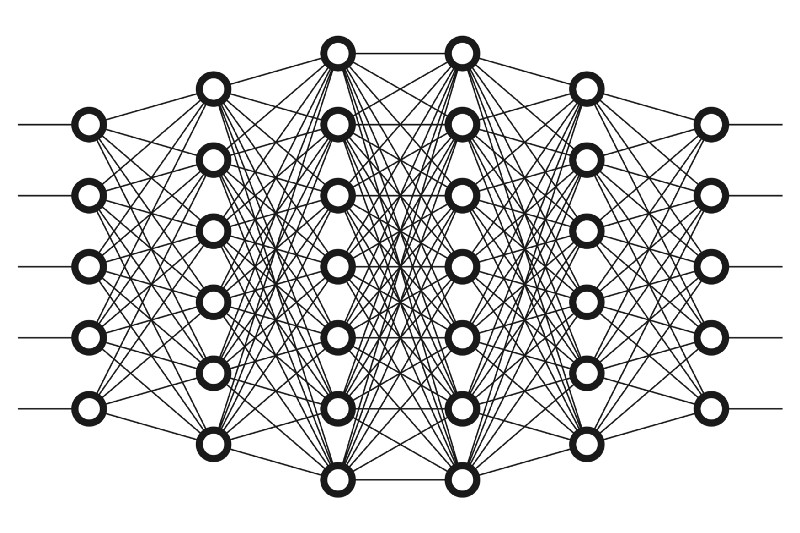
\includegraphics[width=0.6\textwidth]{figs/neuralnetwork.jpeg}
    \caption{Overly simplified view of a neural network composed of multiple neurons, in this case organized in an input layer, four fully-connected hidden layers, and an output layer. Source: datanami.com.}
    \label{fig:neuralnetwork}
\end{figure}

\subsection{Neuron}

A neuron is a computational unit parameterized by a weight vector $W$ and bias scalar $b$, which takes as input $x \in \mathbb{R}^{n}$ and outputs a hypothesis $h_{W,b}(x) = g(\sum^{i=1}_{n} W_{i}x_{i} + b) = g(W^Tx + b)$ that is activated by some (usually non-linear) function $g \colon \mathbb{R} \to \mathbb{R}$ called the activation function.

The activation function $g$ is what characterizes the neuron. If the activation function is the step function

$$
g(x) =
\begin{dcases}
    1,& \text{if } z \geq \theta\\
    0,& \text{if } z < \theta
\end{dcases}
$$

the neuron is reduced to the perceptron presented in 1950-1960 by \citeauthor{perceptron} \cite{perceptron}.

A sigmoid function is any bounded, differentiable, real function (e.g. logistic, tanh).

$$
g(x) = \frac{1}{1 + e^{-x}}
$$

ReLU is the abbreviation of rectified linear unit, which applies the non-saturating activation function $g(x)=\max(0,x)$. It effectively removes negative values from an activation map by setting them to zero. It increases the nonlinear properties of the decision function and of the overall network without affecting the receptive fields of the convolution layer. ReLU is preferred because it trains the neural network faster without a significant penalty to generalization accuracy.[62]

Other functions are also used to increase nonlinearity, for example the saturating hyperbolic tangent $g(x)=\tanh(x)$, $g(x)=|\tanh(x)|$, and the sigmoid function $\sigma (x)=(1+e^{-x})^{-1}$.

An $L$-layer neural network's activations can be recursively defined

$$
a^{l} =
\begin{dcases}
    f(W^{l-1}a^{l-1} + b^{l-1}),& \text{if } 1 < l \leq L\\
    x,              & \text{if } l = 1
\end{dcases}
$$

Let us also define the weighted inputs to the activation function, which is of importance when deriving the backpropagation equations.

$$
z^{l} = W^{l-1}a^{l-1} + b^{l-1}
$$

% TODO: https://cs231n.github.io/convolutional-networks/#conv
\section{Convolutional Neural Network}

A \ac{CNN} is a class of deep, feed-forward artificial neural network, originally designed for computer vision problems where it is most popular. A \ac{CNN} consists of an input and an output layer, as well as multiple hidden layers. The hidden layers of a \ac{CNN} are typically comprised of:

\begin{itemize}
    \item Convolutional base composed by a stack of convolutional and pooling layers. Convolutional layers comprise a set of n independent filters which are independently convolved with the input volume to obtain an output volume of n feature maps. Pooling layers progressively reduce the spatial size of an input volume to reduce the amount of parameters and computation in the network. Pooling layers operate on each feature map independently. The main goal of the convolutional base is to generate features from the image.
    \item Classifier composed by fully connected layers. The main goal of the classifier is to classify the image based on the detected features. A fully connected layer is a layer whose neurons have full connections to all activation in the previous layer.
\end{itemize}

For a particular feature map (the output received on convolving the image with a particular filter is called a feature map), each neuron is connected only to a small chunk of the input image and all the neurons have the same connection weights.

Two key ideas in convolutional neural networks:

\begin{itemize}
    \item Parameter sharing is sharing of weights by all neurons in a particular feature map.
    \item Local connectivity is the concept of each neural connected only to a subset of the input image (unlike a neural network where all the neurons are fully connected)
\end{itemize}

This helps to reduce the number of parameters in the network and makes the computation more efficient.

To summarize, a convolutional layer:

\begin{enumerate}
    \item Accepts a volume of size $W_1 \times H_1 \times D_1$
    \item Requires four hyperparameters:
    \begin{enumerate}
        \item Number of filters $K$,
        \item their spatial extent $F$,
        \item the stride $S$,
        \item the amount of zero padding $P$.
    \end{enumerate}
    \item Produces a volume of size $W_2 \times H_2 \times D_2$ where:
    \begin{enumerate}
        \item $W_2 = H_2 = \frac{W_1 - F + 2P}{S} + 1$
        \item $D_2 = K$
    \end{enumerate}
    \item With parameter sharing, it introduces $F F D_1$ weights per filter, for a total of $(F F D_1) K$ weights and $K$ biases.
    \item In the output volume, the $d$-th depth slice (of size $W_2 \times H_2$) is the result of performing a valid convolution of the $d$-th filter over the input volume with a stride of $S$, and then offset by $d$-th bias.
\end{enumerate}

LeNet \cite{lenet}, in figure \ref{fig:lenet}, is widely considered to be the first successful application of \ac{CNN}, when \citeauthor{lenet} used backpropagation to automatically learn the kernels of convolutions rather than the laborous hand-designed systems that came before it.

\begin{figure}[ht]
    \centering
    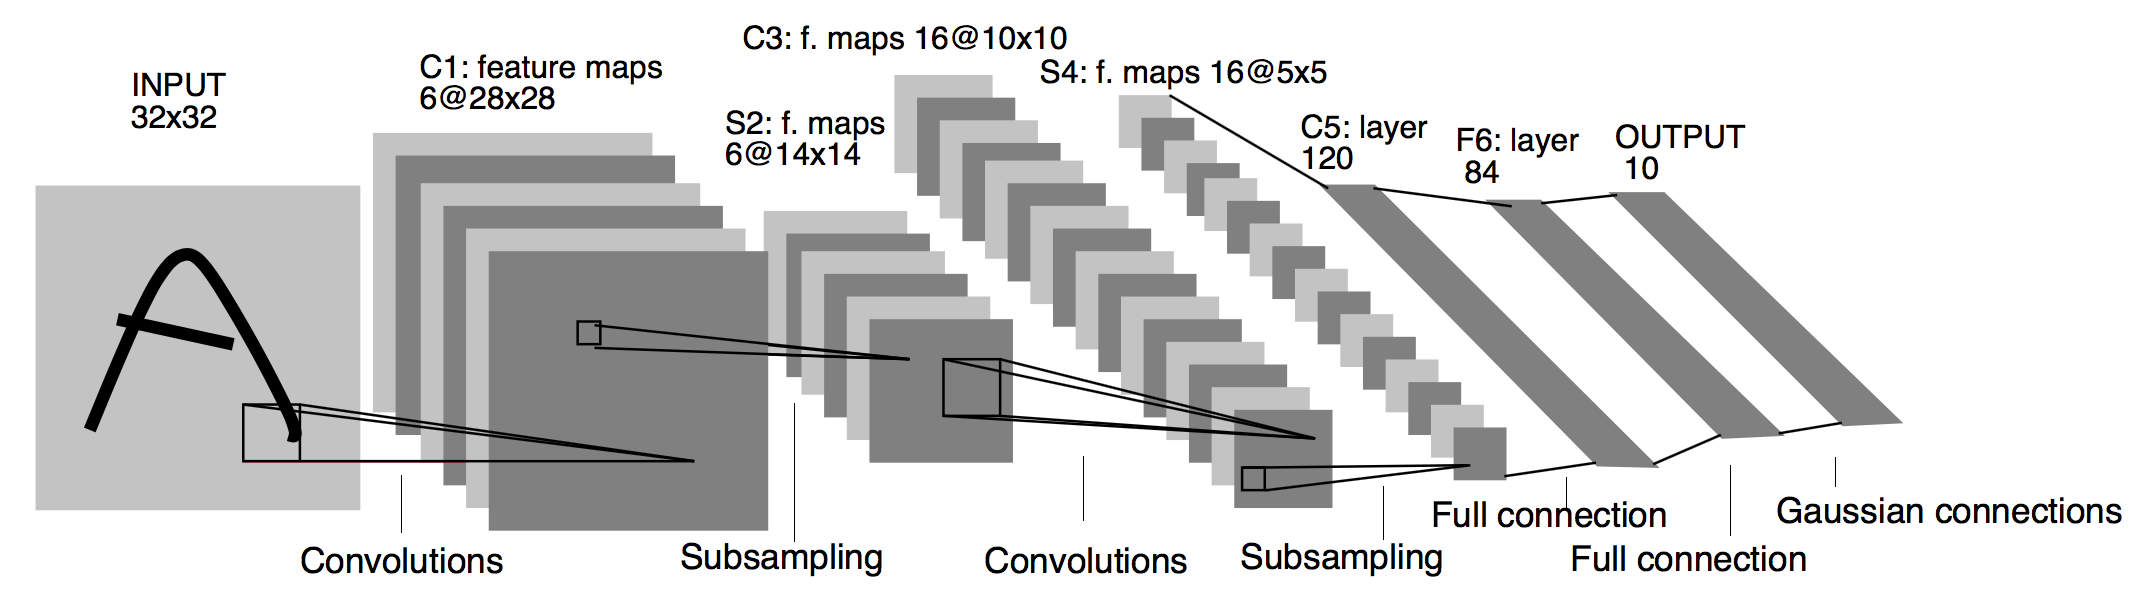
\includegraphics[width=0.5\textwidth]{figs/lenet.png}
    \caption{LeNet}
    \label{fig:lenet}
\end{figure}

AlexNet \cite{alexnet} won the \ac{ILSVRC} \cite{imagenet} in 2012 by a very large margin, introducing a breakthrough in computer vision which further proved that learned features could be better than hand-designed features chosen heuristically. The network, pictured in figure \ref{fig:alexnet}, employed an 8-layer \ac{CNN} that stacked many convolutional layers (immediatelly followed by pooling layers) producing progressively smaller convolutional windows, topped off by two fully-connected layers with 4096 outputs and finally a softmax layer for classification in ImageNet. In its design they also used Dropout regularization and the ReLU activation function, which today are very popular and essential tools in deep learning.

\begin{figure}[ht]
    \centering
    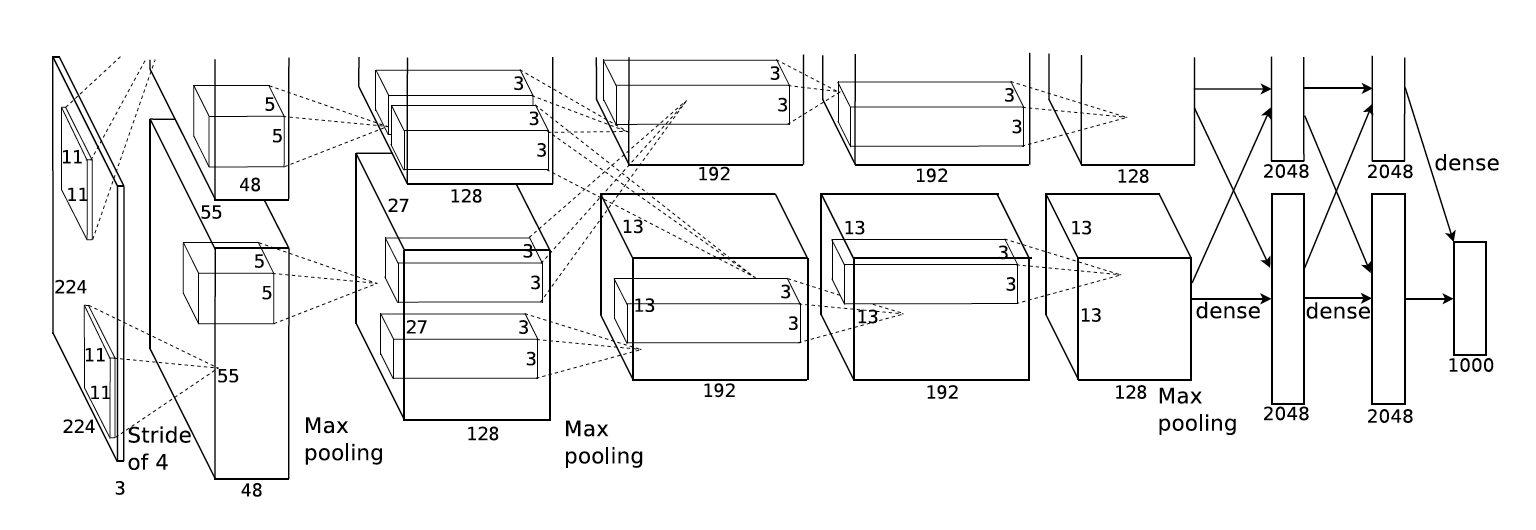
\includegraphics[width=0.6\textwidth]{figs/alexnet.png}
    \caption{AlexNet}
    \label{fig:alexnet}
\end{figure}

Later the \ac{VGG} designed an architecture (illustrated in figure \ref{fig:vgg16}) that used repeated blocks of layers to build progressively more abstract features, shifting thinking in terms of layers to blocks. This basic building block consists of a convolutional layer with padding to maintain resolution, a nonlinearity (i.e. ReLU), pooling for downsampling the features. In the original VGG16 paper \cite{vgg16} the authors employed $3 \times 3$ convolutions and $2 \times 2$ max pooling with stride $S = 2$, essentially halving the resolution after each one of these blocks.

\begin{figure}[ht]
    \centering
    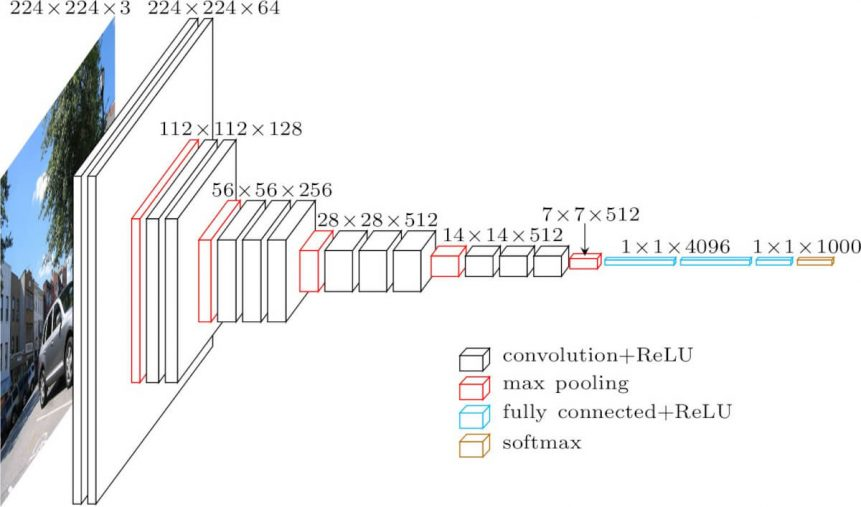
\includegraphics[width=0.6\textwidth]{figs/vgg16.jpg}
    \caption{VGG16}
    \label{fig:vgg16}
\end{figure}

GoogLeNet \cite{inceptionv1} (also known as Inception V1) won the \ac{ILSVRC} \cite{imagenet} in 2014 which introduced the Inception block that establishes four parallel paths that use convolutional layers of different windows and max pooling layers. Furthermore it exhibited lower computational complexity when compared to other models with similar generalization performance. This influenced many later versions of Inception \cite{inceptionv2_3}\cite{inceptionv4}, namely Inception V3 as illustrated in figure \ref{fig:inceptionv3}.

\begin{figure}[ht]
    \centering
    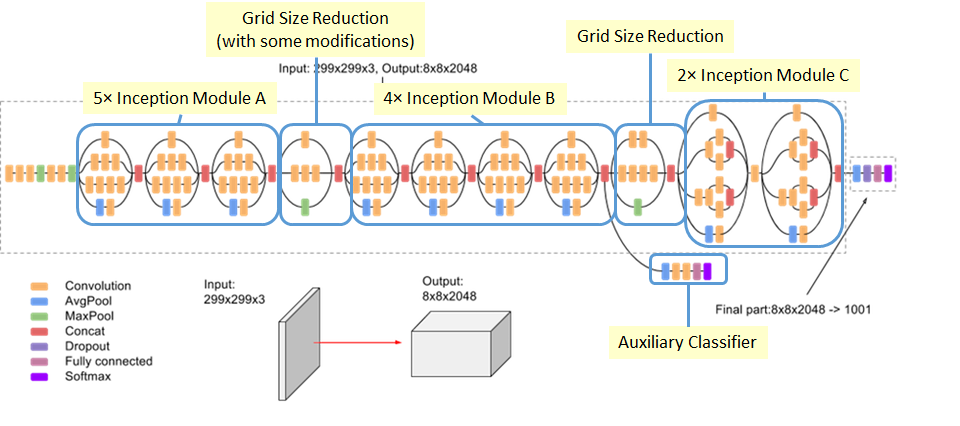
\includegraphics[width=0.6\textwidth]{figs/inceptionv3.png}
    \caption{Inception V3}
    \label{fig:inceptionv3}
\end{figure}

More recently \citeauthor{resnet} have pushed the state-of-the-art by introducing residual neural networks \cite{resnet}. Motivated by avoiding the problem of vanishing gradients, residual networks allow the use of skip connections (or short cuts, as pictured in figure \ref{fig:resnet50}) to arbitrarily jump over layers (effectively reusing activations from previous layers in its forward pass) which significantly speeds up learning by reducing the impact of vanishing gradients since there are less layers to backpropagate through. An ensemble of these networks achieved 3.57\% error on ImageNet, a result which won 1st place on \ac{ILSVRC} 2015.

\begin{figure}[ht]
    \centering
    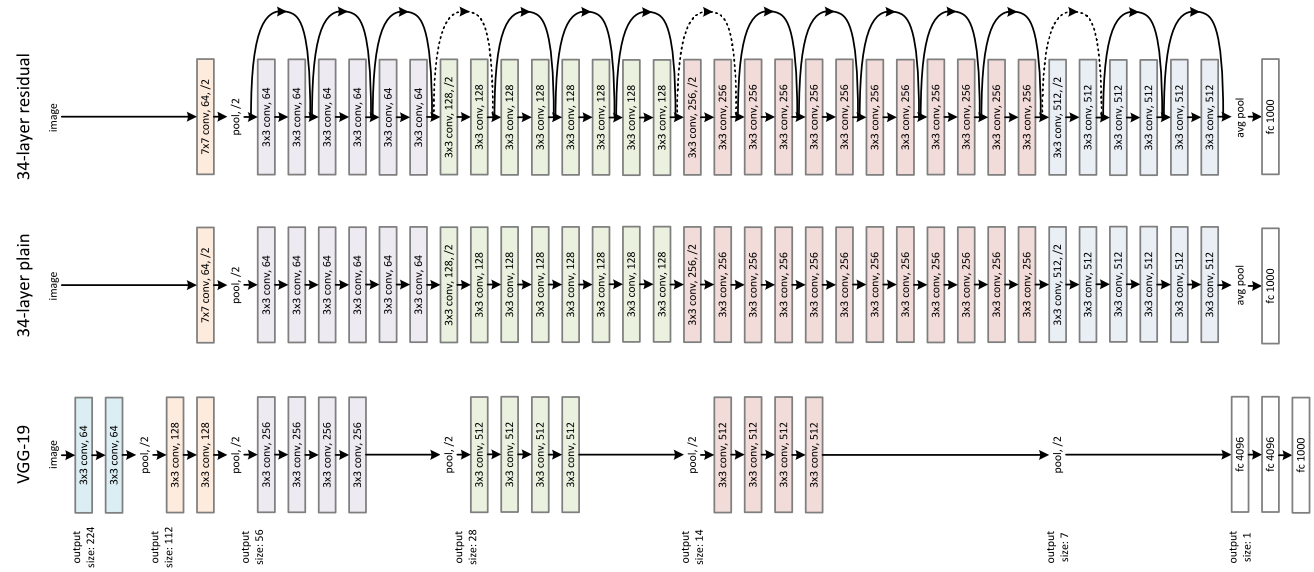
\includegraphics[width=0.7\textwidth]{figs/resnet50.png}
    \caption{Comparison between ResNet-50 and more traditional architectures, illustrating how residual networks avoid the vanishing gradient problem.}
    \label{fig:resnet50}
\end{figure}

\section{Transfer Learning}
\label{section:transferlearning}

Supervised training of deep neural networks requires vast amounts of labeled data, which is very expensive and time consuming in itself, as well as immense computational and time resources which is often equally or more expensive. In practice, transfer learning emerges as a technique that can be used to reduce the costs or time constraints of training these deep neural networks.

Transfer learning is a machine learning technique that seeks to leverage (or transfer) the knowledge gained from solving one problem to another (ideally related) problem \cite{deeptransferlearning}. In the context of deep neural networks it means to transfer the weights of a model trained on a very large dataset (e.g. ImageNet \cite{imagenet}) and re-purpose them for another model.

In image classification problems \ac{CNN} models are used to build progressively more specific feature maps in layers, where lower layers represent abstract, problem independent features (e.g. squares, circles) and higher layers represent specific, problem dependent features (e.g. car, dog). Transfer learning seeks to exploit and take advantage of this construct. In practice, transfer learning for current state-of-the-art image classification techniques boils down to:

\begin{enumerate}
    \item choosing up to which layers should features be extracted
    \item connecting it to a classifier
    \item deciding which layers' weights should be trained (i.e. updated during gradient descent) and which should remain frozen (i.e. not updated during gradient descent)
\end{enumerate}

The classifier is commonly based on:

\begin{itemize}
    \item Fully connected layers;
    \item Global average pooling;
    \item SVM.
\end{itemize}

\subsection{Transfer Learning by Total Feature Extraction}

In the simplest scenario:

\begin{enumerate}
    \item extract all the convolutional layers of the pre-trained model
    \item freeze the weights of all the extracted layers
    \item build a classifier on top of the extracted features and only train the weights of the classifier layers
\end{enumerate}

\subsection{Transfer Learning by Partial Feature Extraction}

When the source and target domains are not very similar, extracting higher layers will yield features that are too specific to the source domain. For example, if the source domain is cars but the target domain is dogs, then the higher layers likely represent features very specific to dogs (e.g. dog eyes, dog tails, dog legs), whereas some arbitrary middle layer might represent more abstract shape-like features that can still be used as a solid starting point for the cars domain.

For this reason it is often counter-productive to extract all the features. Instead features can be extracted up to an arbitrary middle layer which likely represents more useful features that are still relevant for the target domain. The precise point up to which features should be extracted needs to be studied and tested empirically for each problem and chosen based on whichever yields the highest generalization performance.

Like the previous strategy, the classifier is built on top of the extracted features and only the weights of the classifier layers are trained.

\subsection{Transfer Learning by Fine-Tuning}

The weights of the extracted layers (regardless if they were all extracted or only partially) do not all need to remain frozen. Given sufficient computational and time resources, further training the weights of the extracted layers can yield even higher generalization performance because we are, in some sense, fine-tuning the weights of the extracted features to better fit the target dataset.

For this fine-tuning one should be very careful and make sure to use a very slow (i.e. low) learning rate so as to not suddenly disrupt the learned features, because we are actually updating weights transferred from another model.

\section{Ensemble Learning}

Ensemble learning is a machine learning paradigm that designs models by combining other models into a single more complex and presumably more accurate model. In ensemble learning theory we refer to these building block models as weak learners because they usually suffer from high bias or high variance, which are combined in such a way to reduce the bias and variance into a final ensemble model called a strong learner.

There are three major ensemble learning methods: bagging, boosting, and stacking.

\subsection{Bagging}

Bagging, short for bootstrap aggregation, focuses on reducing variance and relies on $L$ approximately i.i.d. subsamples of the data (called bootstrap samples) to fit $L$ weak learners $h_1(x), h_2(x), \ldots, h_L(x)$ and aggregate or average them through some function $H(x)$ which e.g.

\begin{enumerate}
    \item in a regression problem can literally be the average of the predictions of the weak learners, sometimes referred to as soft voting, i.e. $H(x) = \frac{1}{L} \sum_{i=1}^{L} h_i(x)$
    \item in a classification problem can be to just take the mode of the predictions of the weak learners, often called hard voting, i.e. $H(x) = \mode{(h_1(x), h_2(x), \ldots, h_L(x))}$
\end{enumerate}

Perhaps the biggest advantage of bagging is that the the $L$ weak learners can be fit independently and in parallel, considerably speeding up research iterations.

\subsection{Boosting}

Boosting fits multiple models sequentially such that the model being fit at a given iteration gives more importance to samples that were previously predicted with high error, thus resulting in a strong learner with lower bias than its weak learners.

Adaptive boosting (also known as AdaBoost) \cite{adaboost} combines the output of its $T$ weak learners into a weighted sum that represents the final output and is of the form

$$
H_T(x) = \sum_{t=1}^{T} \alpha_t h_t
$$

Rather than optimizing for the optimal set of weights $\alpha_t$ and weak learners $h_t$, AdaBoost takes an iterative approach. Essentially, at each iteration $t$, a weak learner $h_t$ is chosen and weighted $\alpha_t$ to minimize the training error $E_t$ of the $t$-th boosting classifier

$$
E_t = \sum_{t=1}^{T} E[H_{t-1}(x_t) + \alpha_t h_t(x_i)]
$$

\subsection{Stacking}

Rather than combining the weak learners using some arbitrary pre-determined scheme, stacking learns this combination by training a meta-model based on the weak learners' predictions, which can even be done in multiple layers.

Stacking often works well with heterogeneous weak learners, i.e. different algorithms. For example, our weak learners could consist of \ac{KNN}, \ac{SVM}, and decision tree models. Then, the outputs of the weak learners could be taken as inputs for an \ac{ANN} to learn the meta-model based on their predictions.

The data that is used to train the weak learners is not relevant for training the meta-model. Thus we need to split the data in two folds: one for training the weak learners and another for training the meta-model. An obvious immediate drawback is that we only have a fraction of the data available for training the meta-model and vice versa.

\section{Deep Learning Hardware}

Deep learning is very computationally intensive in itself and even more so when we want to run multiple experiments with hyperparameters or even completely different architectures.

\ac{CNN}, the core of most state-of-the-art deep learning applied to computer vision, are computationally complex and embarassingly parallel \cite{chang2017} which the architecture of general purpose \ac{GPU} are appropriate for \cite{gpu} and for which libraries like cuDNN \cite{cudnn} were developed to further leverage the characteristics of \ac{GPU} into even bigger performance improvements.

There is a growing demand for domain-specific hardware designed specifically for the computations necessary in neural network training and inference, like Google's TPU custom ASIC \cite{tpu}, which naturally can achieve major improvements in cost-energy-performance when compared to general purpose hardware like \ac{GPU} that were originally designed for the demands of computer graphics which coincidentally also serve deep learning reasonably well. Nonetheless, \ac{GPU} remain the best cost-effective commodity hardware for this type of computation, especially when not working at the scale of companies like Google and Facebook. In a typical scenario, the CPU does little useful computation in a deep learning application where most of the computation is delegated to the GPU.

% TODO: write more

\section{Deep Learning Software Frameworks}

TensorFlow is an open source software library for numerical computation using data flow graphs. The graph nodes represent mathematical operations, while the graph edges represent the tensors that flow between them. This flexible architecture enables you to deploy computation to one or more CPU or GPU in a desktop, server, or mobile device without rewriting code \cite{tensorflow}.

Keras is a high-level neural networks API, written in Python and capable of running on top of TensorFlow, CNTK or Theano. It was developed with a focus on fast experimentation which enables easy and fast prototyping through user friendliness, modularity, and extensibility. This API was more recently adopted by TensorFlow itself in the tf.keras namespace which is given a lot more attention in TensorFlow 2.0 (following the criticism of TensorFlow's convoluted API).

% TODO: write more

\chapter{State of the Art}
\label{chapter:sota}

This chapter reviews current state-of-the-art results in skin lesion classification and medical image analysis in general to get an overview of the work related to this dissertation and to establish a baseline for comparison.

\section{Transfer Learning Approaches}

\citeauthor{Brinker2018} \cite{Brinker2018} present the first systematic review of the cutting edge in lesion classification with deep convolutional neural networks, which remains the fundamental technique in state-of-the-art results. They review 13 papers that use \ac{CNN}, most of which transfer weights from networks trained on \ac{ILSVRC} to the target task, which speeds up training and reduces costs by leveraging previous knowledge. In conclusion they note that \ac{CNN} are currently the state-of-the-art in skin lesion classification and that transfer learning is a very effective approach, but that it was rather difficult to compare results given the heterogeneity of datasets (some of which are not public) making reproduceability difficult. This motivated the initiative by the ISIC Archive to collect and uniformize data as well as organize challenges to push new results.

In \citeyear{nature2017} \citeauthor{nature2017} \cite{nature2017} achieved perhaps the most famous result in skin lesion classification using deep learning, making it to the Nature scientific journal. Their dataset combines biopsy-proven data from the ISIC Archive, Edinburgh Dermofit Library, and the Stanford Hospital, totalling an astonishing 129450 samples (after going through data augmentation of random flips, rotations, crops) which remains one of the biggest efforts in data collection in the area. They build an undirected graph connecting images that were deemed to be similar and made sure that the connected components of this graph were separated and distributed between the train, validation, and test sets in order to create a more effective and diverse split of the data. The authors follow a transfer learning approach by leveraging the weights of the InceptionV3 network trained on ImageNet, on top of which they build their own classifier and fine-tune previous layers carefully using the RMSProp optimizer. They evaluate the performance of the network by pitting it against 21 board-certified dermatologists on biopsy-proven medically-relevant cases of keratinocyte carcinomas versus benign seborrheic keratoses and malignant melanomas versus benign nevi, attaining performance on par with experts.

\citeauthor{menegola2017} \cite{menegola2017} went back to the ISIC 2016 lesion classification challenge to try to obtain better results and employed a transfer learning approach to leverage weights from VGG-16 and VGG-M networks originally trained on ImageNet and fine-tune the network on a dataset comprised of data from the ISIC 2016 challenge and the Interactive Atlas of Dermoscopy (augmented by randomly scaling, rotating or flipping the samples) which they train for 60 epochs using \ac{SGD} with momentum and L2 regularization to obtain a set of features on top of which they train an SVM classifier. They report results on the test set of the ISIC 2016 challenge, achieving 0.807 AUC with the deeper VGG-16 model. Their results further show that in really difficult cases their model is not very confident in its prediction, which suggests that, for the time being, current technology is better used as a reference to support and explain the diagnosis human doctors' rather than as a complete diagnosis framework.

\subsection{ISIC 2017 Part 3: Lesion Classification}

In part 3 of the ISIC 2017 \cite{isic2017} challenge participants were asked to develop two binary classifiers to distinguish between:

\begin{itemize}
    \item melanoma vs nevus and seborrheic keratosis
    \item seborrheic keratosis vs nevus and melanoma
\end{itemize}

Participants were given a training set of 2000 images (374 melanoma, 254 seborrheic keratosis, and the remaining 1372 benign nevi), a validation set of 150 images and a test set of 600 images. The images were of questionable quality and required a lot of preprocessing effort, which they could also complement by gathering their own data. Participants were ranked and awarded based only on AUC, but other metrics were reported for scientific completeness.

% first place
First place was a joint effort between Casio and Shinshu University presented by Kazuhisa Matsunaga et al\cite{isic2017first}. In their work they adopted ensembles of their own variant of ResNet-50 that they trained presumably end-to-end (using RMSProp\cite{rmsprop} and AdaGrad\cite{adagrad}) on data from the challenge as well as data they gathered independently, which was normalized in such a way to exploit color constancy and of which multiple geometric transformations were input in parallel to the networks.

The metadata available in the training set showed that melanoma and seborrheic keratosis were both uncommon in young ages. From this observation they implemented a simple thresholding by age, which improved performance for seborrheic keratosis classification from 0.957 to 0.960 AUC in cross-validation but not for melanoma classification. They noted that a more careful thresholding implementation is necessary from a clinical point of view. In the end, the mean performance of the two classifiers on the validation set was 0.958 AUC and, after the paper was published, 0.911 on the test set.

% second place
Iván from the Universidad Carlos III de Madrid \cite{isic2017second} got second place by designing a very complete automatic diagnosis system where a dermoscopic image goes through:

\begin{enumerate}
    \item A segmentation network based on \ac{FCN} \cite{fcn} to generate a binary mask outlining the area actually occupied by the lesion
    \item A data augmentation module to generate random label-invariant views of the original dermoscopic image through rotations and crops.
    \item A structure segmentation network that produces binary masks for 8 heuristically designed structures (dots, reticular patterns and pigmented networks, homogeneous areas, regression areas, blue-white veil, streaks, vascular structures, and other unspecific patterns) that expert dermatologists find important for a diagnosis
    \item A classification network based on transfer learning from ResNet-50 \cite{resnet} that takes into consideration the structures identified by the structure segmentation network as well as the original dermoscopic image.
\end{enumerate}

This effort resulted in AUC score of 0.910 on the test set, thus earning second place.

% third place
Third place was an effort by Afonso Menegola et al \cite{isic2017third} from RECOD Lab. who collected several datasets which they cleaned and filtered, resulting in two sets of 9640 and 7544 images with differing performances on the two different binary classification tasks that they decided to keep in consideration throughout their experiments. They adopted a transfer learning approach and decided to focus on ResNet-101 and Inception-V4 models trained on ImageNet on top of which they experimented with:

\begin{itemize}
    \item Curriculum learning scheme in which they schedule the samples during training such that easier samples are batched first and harder samples are batched later. However in practice this was worse than a traditional learning scheme.
    \item Training data and testing data augmentation by applying label-invariant random transformations such as crops, flips, etc. that ended up significantly improving performance (which the authors already knew from experience).
    \item Meta-learning scheme to take into consideration the decision of multiple models (even by simply averaging the output probabilities) gave the best results on the official validation AUC, even when compared to the single best model.
    \item Normalizing the inputs to Inception networks by subtracting the average pixel value significantly improved performance, but further dividing by the standard deviation gave worse results than baseline.
\end{itemize}

Their final submission was a meta model that combined seven models based on Inception and ResNet networks trained on distinct datasets which were then stacked in a meta-learning layer based on SVM. In the end they placed third by getting an AUC score of 0.908 on the test set.

% others
Also worth noting is

\begin{itemize}
    \item \citeauthor{isic2017li} \cite{isic2017li} who present novel multi-scale fully convolutional residual networks (based on FCRN-88 \cite{fcrn}) trained on datasets augmented differently (which empirically proved to offer better performance) whose outputs are interpolated to the original scale and summed up to yield what the authors call possibility maps which are further refined by taking into a consideration a distance map representing the importance of each pixel. For comparison they also ran experiments with AlexNet, VGG16, ResNet-50, ResNet-101, Inception-v3, but their custom network outperformed them all with an AUC score of 0.912 as evaluated on the ISIC 2017 dataset.
    \item \citeauthor{yang2017} \cite{yang2017} whose work propose a multi-task learning scheme where lesion segmentation and classification are solved simultaneously by constructing a model that builds feature maps using \ac{CNN} which then branches out into 3 parallel paths whose outputs individually do segmentation, melanoma binary classification, and seborrheic keratosis binary classification, but training is performed as if it was a single network optimizing parameters as usual. They achieve an AUC score of 0.926.
\end{itemize}

\subsection{ISIC 2018 Part 3: Lesion Classification}

In part 3 of the ISIC 2018 challenge participants were asked to develop a classifier to distinguish between:

\begin{itemize}
    \item Melanoma
    \item Melanocytic nevus
    \item Basal cell carcinoma
    \item Actinic keratosis
    \item Benign keratosis
    \item Dermatofibroma
    \item Vascular lesion
\end{itemize}

The provided training data comes from the HAM10000 Dataset \cite{ham10000}, which was acquired with many different dermatoscopes, from most anatomic sites, from a historical sample of patients presented for skin cancer screening, from many different institutions, with the proper approval. Diagnosis ground truth labels were established by:

\begin{itemize}
    \item Histopathology
    \item Reflectance confocal microscopy
    \item Lesion did not change during digital dermatoscopic follow up over two years with at least three images
    \item Consensus of at least three expert dermatologists from a single image
    \item Histopathology confirmation in cases of malignancy
\end{itemize}

Just like in the 2017 edition, participants could, of course, complement the training data by gathering their own, but this time they were ranked based on normalized multi-class accuracy metric.

In the 2018 edition \citeauthor{isic2018first} \cite{isic2018first} won first, second, and third place, attaining, respectively, a balanced multiclass accuracy of 0.885, 0.882, and 0.871 (which still beat fourth place by a margin of 2\%). In their work they combined data from the competition's HAM10000 dataset, the ISIC Archive, and other proprietary data, which were preprocessed using the Shades of Gray method to normalize images from different sources and contexts. Further in their data pipeline they augment training data by performing random horizontal flips, random rotations of ${0, 90, 180, 270}$ degrees, change brightness, saturation, and contrast by a random factor in the range $[0.9, 1.1]$. Their models were based on transfer learning from models trained on ImageNet like InceptionV3, ResNet-50, Squeezenet, Densenet, and others, of which they picked the best-performing and ensembled them in a stacking scheme.

The authors note that a large ensemble of models like theirs is not practical in production because of the high computational cost associated with infering the prediction of a given input for all models in the ensemble. For this reason, they suggest that constraints on memory usage or \ac{FLOPS} be considered in future challenges.

Noteworthy are also the submissions by

\begin{itemize}
    \item \citeauthor{isic2018milton} \cite{isic2018milton} who also followed an approach based on transfer learning from models of PNASNet-5-Large, InceptionResNetV2, SENet154, InceptionV4 trained on ImageNet, who interestingly noted that in the first few epochs the gradient is very erratic and thus refrained from fine-tuning weights during the first 2 epochs to avoid updating weights towards the wrong direction, in the end achieving a score of 0.76 on the validation set;
    \item \citeauthor{isic2018bissoto} \cite{isic2018bissoto} (who won 3rd place in the 2017 edition) which transfered knowledge from models of InceptionV4, ResNet-152, and DenseNet-161 trained on ImageNet, by training with online data augmentation (e.g. random crops, flips, rotations, shears, color transformations), \ac{SGD} with the learning rate being decreased by a factor of 10 whenever validation loss didn't improve for 10 epochs, eventually building an average of 15 models trained only with the challenge data that attained a score of 0.803.
\end{itemize}

\section{Hybrid Learning Techniques}

Clearly the large majority of the work in skin lesion classification follows a transfer learning approach, presumably because of how cost-effective it is (especially for smaller research teams). Nonetheless there has been some research that explore other techniques in addition to transfer learning.

\citeauthor{hybrid2} \cite{hybrid2} present an approach that extracts features from

\begin{itemize}
    \item a \ac{VGG} network originally trained on ImageNet
    \item unsupervised feature learning using sparse coding
\end{itemize}

and respectively trains two non-linear \ac{SVM} (using a histogram intersection kernel and sigmoid feature normalization) whose outputs are mapped to probabilities at a 50\% threshold and fused together using unweighted score averaging. They compare this against a more classical ensemble approach using only hand-coded low-level features, which used to be the state-of-the-art but is now significantly less performant at 0.715 accuracy on their test set (versus the 0.739 accuracy of the hybrid approach).

The work by \citeauthor{hybrid1} \cite{hybrid1} combines different techniques into a similar (but more extensive) classification framework that basically:

\begin{enumerate}
    \item extracts various features across two input scales (an area cropped around the segmented lesion, and the entire original dermoscopic image)
    \begin{itemize}
        \item hand-engineered rule-based features like color histogram, edge histogram, and color local binary patterns;
        \item unsupervised learning features from a sparse coded representation;
        \item features extracted from two deep residual networks trained on ImageNet and fine-tuned on the target dataset;
        \item the segmentation produced by their U-Net segmentation network is also used as a shape descriptor feature.
    \end{itemize}
    \item trains non-linear \ac{SVM} to learn a classifier for each extracted set of features;
    \item averages the output of each classifier in an ensemble to produce a final classification.
\end{enumerate}

When compared to an average of 8 dermatologists' predictions on 100 test images, they produce a higher accuracy and specificity evaluated at an equivalent sensitivity.

\chapter{Methodology}
\label{chapter:methodology}

This section describes, in detail, the methodology behind this dissertation's research objectives, namely:

\begin{itemize}
    \item Dataset description, preprocessing steps, and augmentation techniques;
    \item Software stack used to describe said experiments in code;
    \item Computational resources used to execute the experiments.
\end{itemize}

\section{Data}

The \ac{ISIC} 2017: Skin Lesion Analysis Towards Melanoma Detection grand challenge datasets \cite{isic2017} provides a training set with 2000 samples (divided into three classes: 374 melanoma, 254 seborrheic keratosis, and 1372 nevus), a validation set with 150 samples, and a test set with 600 samples. However training deep neural networks for skin lesion classification requires vast amounts of high quality, reliably labeled and verified data - a set of requirements which this dataset did not meet with confidence.

The \ac{HAM10000} \cite{ham10000} dataset is an effort to boost research on automated diagnosis of dermatoscopic images that focuses on the quality and reliability of the large volume of data that is so important for successful deep learning. The extracted images (where the lesion is centered if necessary) go through an extensive semi-automatic process that filters out non-dermoscopic imaging and unreliable diagnoses, after which they are submitted to a manual review to further confirm its quality.

The datasets from the \ac{ISIC} 2018 grand challenge \cite{isic2018} were largely based on \ac{HAM10000} that was already very high quality, which meant the data preprocessing needs would be much lower compared to the previous years' editions where all these quality guarantees had to be independently ensured by the competitors. The \ac{ISIC} 2018 datasets are therefore adequate for running these experiments.

\subsection{Preprocessing}
\label{subsection:preprocessing}

The images in the dataset undergo a number of preprocessing steps:

\begin{enumerate}
    \item Most readily available pretrained models are of network architectures whose input tensor is of square dimensions (e.g. $224 \times 224 \times 3$). Since our dataset's images are of distinct non-square dimensions, it is necessary to resize them to a square. However, resizing them all naively to the network's input tensor dimensions without regards to the image's aspect ratio means that the input fed to the network is of varying distinct aspect ratios which does not constitute a good start. Therefore, the first step is to crop an arbitrarily-sized square of the center of the image which will likely (and, in fact, does) capture the skin lesion.

    \begin{listing}[ht]
    \begin{minted}{python}
    def _crop(img):
        width, height = img.size
        if width == height:
            return img

        length = min(width, height)

        left = (width - length) // 2
        upper = (height - length) // 2
        right = left + length
        lower = upper + length

        box = (left, upper, right, lower)
        return img.crop(box)
    \end{minted}
    \caption{Function that crops a given image to a square crop of the center of the original image.}
    \label{code:crop}
    \end{listing}

\item Resize the images to the target networks' input dimensions $224 \times 224 \times 3$ and $299 \times 299 \times 3$. We resize (using nearest-neighbor interpolation) them as soon as possible in the data pipeline in order to reduce the computational costs of any subsequent operations on the images.

    \begin{listing}[ht]
    \begin{minted}{python}
    def _resize(img, target_size):
        return img.resize(target_size, PIL.Image.NEAREST)
    \end{minted}
    \caption{Function that resizes a given image to the target dimensions.}
    \label{code:resize}
    \end{listing}

    \item Normalize the luminance and apply a 99\% contrast stretch to reduce the negative effect of changes in illumination and acquisition devices that alter the color of images \cite{colorconstancy}.

    \begin{listing}[ht]
    \begin{minted}{python}
    def _correct(img):
        img_y, img_b, img_r = img.convert('YCbCr').split()

        img_y_np = np.asarray(img_y).astype(float)

        img_y_np /= 255
        img_y_np -= img_y_np.mean()
        img_y_np /= img_y_np.std()
        scale = np.max([np.abs(np.percentile(img_y_np, 1.0)),
                        np.abs(np.percentile(img_y_np, 99.0))])
        img_y_np = img_y_np / scale
        img_y_np = np.clip(img_y_np, -1.0, 1.0)
        img_y_np = (img_y_np + 1.0) / 2.0

        img_y_np = (img_y_np * 255 + 0.5).astype(np.uint8)

        img_y = PIL.Image.fromarray(img_y_np)

        img_ybr = PIL.Image.merge('YCbCr', (img_y, img_b, img_r))
        return img_ybr.convert('RGB')
    \end{minted}
    \caption{Function that normalizes the luminance of an image and applies a 99\% contrast stretch.}
    \label{code:correct}
    \end{listing}
\end{enumerate}

\subsection{Augmentation}
\label{subsection:augmentation}

In our binary classification task (melanoma vs non-melanoma) the $m = 10015$ samples in the training set are highly imbalanced (illustrated in figure \ref{fig:classimbalance}):

\begin{itemize}
    \item the majority class has $|S_{maj}| = 8902$ samples, constituting $\frac{8902}{10015} \times 100 = 88.9\%$ of the samples;
    \item the minority class has $|S_{min}| = 1113$ samples, constituting $\frac{1113}{10015} \times 100 = 11.1\%$ of the samples.
\end{itemize}

\begin{figure}[ht]
    \centering
    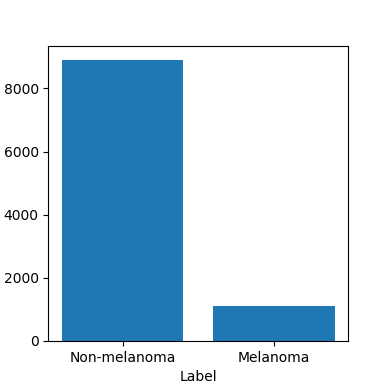
\includegraphics[width=0.5\textwidth]{figs/data_barplot.png}
    \caption{Bar plot of the distribution of the dataset's labels (melanoma or non-melanoma cases).}
    \label{fig:classimbalance}
\end{figure}

We correct this imbalance by oversampling the minority class, while also augmenting the total number of samples to $m' \approx 18000$ to increase the size of the dataset. That means we must augment the minority class by a factor of $\frac{\frac{m'}{2}}{|S_{min}|}$ and the majority class by a factor of $\frac{\frac{m'}{2}}{|S_{maj}|}$. For this augmentation we consider a set $T$ of possible transformations:

\begin{itemize}
    \item Horizontal flip
    \item Vertical flip
    \item 90º rotation
    \item 180º rotation
    \item 270º rotation
\end{itemize}

implemented by \verb|PIL.Image.transpose|\footnote{\url{https://pillow.readthedocs.io/en/stable/reference/Image.html\#PIL.Image.Image.transpose}} with the respective method:

\begin{itemize}
    \item \verb|PIL.Image.FLIP_LEFT_RIGHT|;
    \item \verb|PIL.Image.FLIP_TOP_BOTTOM|;
    \item \verb|PIL.Image.ROTATE_90|;
    \item \verb|PIL.Image.ROTATE_180|;
    \item \verb|PIL.Image.ROTATE_270|.
\end{itemize}

On principle, we did not consider transformations that change the color (e.g. contrast change, channel shift) or size (e.g. zoom) of features because it would unjustifiably allow the network to learn from these potentially misrepresenting features which even an expert human diagnosis would have trouble with.

The final available augmentations are all the $k$-combinations of the set $T$ for $k \in \{1, ..., |T|\}$, in other words all the possible ways in which you can combine the transformations from the set $T$.

\subsection{Split}

The number of variables in the future experiments would quickly lead to a combinatorial explosion of configurations, so to minimize the computational cost of the experiments a fixed validation scheme will be used rather than a cross validation scheme. To compensate for this lack of averaging over multiple folds of the data (which gives statistical confidence in the results), a fixed seed is set for every \ac{PRNG} as in code listing \ref{code:seed}, which in practice means parameters are initialized identically between experiments (providing some level of statistical confidence when making comparisons) and guarantees reproducibility.

\begin{listing}[ht]
\begin{minted}{python}
def seed():
    from random import seed
    seed(1)
    import numpy.random
    numpy.random.seed(2)
    from tensorflow import set_random_seed
    set_random_seed(3)
\end{minted}
\caption{Seed function that is called on every experiment to ensure reproducibility and similar conditions between experiments.}
\label{code:seed}
\end{listing}

The original training set from \ac{ISIC} 2018 is available for direct download, but the validation and test sets are kept private by the organization and are only used internally for reporting performance without actually releasing the data itself. As such, we will split the samples from the training set (which is available for download) into our own training, validation and test sets.

Augmentation, as described previously, results in 17810 samples which are split 85\%-15\% in a stratified fashion to maintain class balance within the splits into:

\begin{itemize}
    \item 15137 training samples, illustrated in figure \ref{fig:data_train};
    \item 2673 test samples, illustrated in figure \ref{fig:data_test}.
\end{itemize}

\begin{figure}[ht]
    \centering
    \includegraphics[width=0.6\textwidth]{../plots/data/train.png}
    \caption{Randomly-sampled images and respective labels of the train set.}
    \label{fig:data_train}
\end{figure}

\begin{figure}[ht]
    \centering
    \includegraphics[width=0.6\textwidth]{../plots/data/test.png}
    \caption{Randomly-sampled images and respective labels of the test set.}
    \label{fig:data_test}
\end{figure}

Since validation is intrinsically part of the training process itself, the validation set is a 15\% split from the training set obtained independently at the start of each training routine (also in a stratified fashion).

\section{Hardware}

Initially, computational resources from \ac{IEETA} were used in very early exploratory research:

\begin{itemize}
    \item Intel® Xeon® Processor E5-2640;
    \item NVIDIA Tesla K40c;
    \item NVIDIA Quadro K4000;
    \item 32GB DDR4 RAM.
\end{itemize}

However, given that it was shared between dozens of other researchers it was deemed not enough for a comfortable and flexible workflow because:

\begin{itemize}
    \item the little amount of memory almost wasn't enough to load the dataset into memory, especially during critically busy times;
    \item the NVIDIA Quadro K4000, with a compute capability of 3.0, was unsupported by the software stack which required a minimum compute capability of 3.7, leaving only a single NVIDIA Tesla K40c to work with.
\end{itemize}

More recently, \ac{LAR}, located in the Department of Mechanical Engineering at the University of Aveiro, has provided access to their deep learning research server codenamed Deeplar:

\begin{figure}[ht]
    \centering
    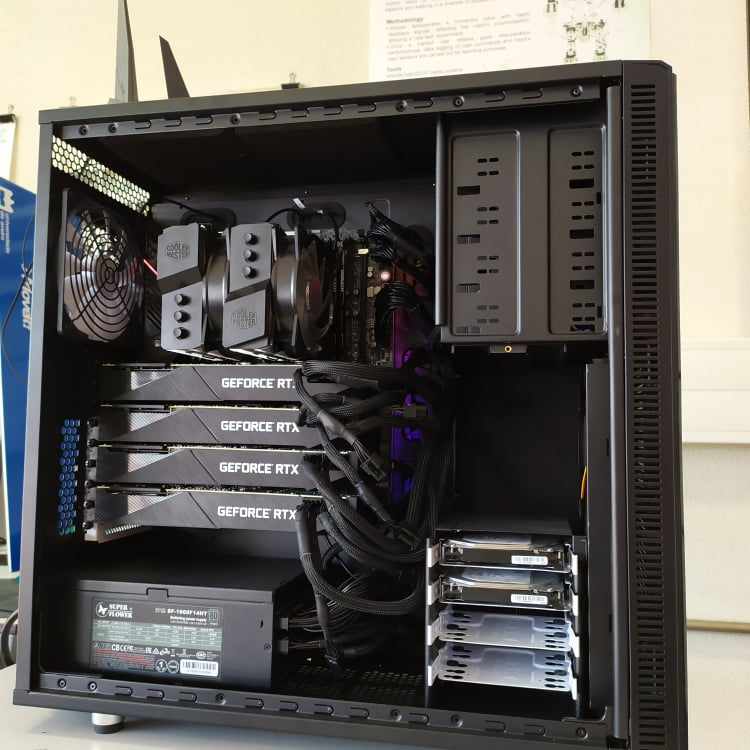
\includegraphics[width=0.4\textwidth]{figs/deeplar.jpg}
    \caption{Deeplar, the deep learning research server at \ac{LAR}}
    \label{fig:deeplar}
\end{figure}

\begin{itemize}
    \item AMD Ryzen™ Threadripper 2950X;
    \item Four NVIDIA GEFORCE® RTX 2080 Ti;
    \item 128GB DDR4 RAM.
\end{itemize}

The latter much more capable server (four state-of-the-art consumer \ac{GPU} and lots of \ac{RAM}) was effectively responsible for running this work's experiments.

\section{Software}

The deep learning research server Deeplar runs on openSUSE Tumbleweed 20191004\footnote{\url{https://software.opensuse.org/distributions/tumbleweed}}, a popular rolling-release GNU/Linux distribution. For interfacing with the \ac{GPU} it has installed CUDA 9.2 \footnote{\url{https://developer.nvidia.com/cuda-zone}} (NVIDIA GPU's proprietary language and API) and cuDNN 7.6.0 \footnote{\url{https://developer.nvidia.com/cudnn}} (a library for working with deep neural networks which most higher level frameworks rely on).

We used Miniconda\footnote{\url{https://docs.conda.io/en/latest/miniconda.html}} to install Conda\footnote{\url{https://conda.io/en/latest/}} which was used to manage a Python 3.6\footnote{\url{https://www.python.org/}} environment which was specifically required for compatibility with TensorFlow. Crucially, the following Python packages and specific versions were used for the development of most of the source code.

\begin{itemize}
    \item TensorFlow\footnote{\url{https://www.tensorflow.org/}} 1.12.0, of which we mostly use the \verb|tf.keras| API, for training and testing the various models;
    \item scikit-learn\footnote{\url{https://scikit-learn.org/}} 0.20.2 for some useful metrics and data splitting methods;
    \item NumPy\footnote{\url{https://numpy.org/}} 1.15.4 for various vector and matrix operations and Pillow\footnote{\url{https://pillow.readthedocs.io/en/stable/}} 5.4.1 for image handling and transformations because of this work's image preprocessing needs.
\end{itemize}

\chapter{Conclusion}
\label{chapter:conclusion}

In this section we present conclusions, final remarks, and point to directions for future work.

Ironically, when compared to end-to-end learning, most transfer learning experiments actually take longer because of the large number of parameters that you end up training anyway



% End of Thesis text ---------------------------------------------------------
% Including files is advised:


%Appendix

\backmatter


%Print all used references

\begingroup
\renewcommand{\bibfont}{\footnotesize}

%Redefine References name
\defbibheading{bibliography}[References]{
	\chapter{#1}
}
\SingleSpacing
\setlength\bibitemsep{8pt}
\printbibliography[heading=bibliography]
\endgroup


%Load appendix
%\include{appendix-a}


\end{document}
